\documentclass[a4paper,11pt]{article}
\usepackage[left=2cm,text={17cm, 24cm},top=3cm]{geometry}
\usepackage[utf8]{inputenc}
\usepackage[czech]{babel}
\usepackage[T1]{fontenc}
\usepackage{times}
\usepackage[hidelinks]{hyperref}
\usepackage{graphicx}
\usepackage{booktabs}
\usepackage{epstopdf}
\usepackage{fancyvrb}
\usepackage[htt]{hyphenat}
\usepackage{amsmath}
\usepackage{float}
\fvset{frame=single,framesep=1mm,fontfamily=courier,fontsize=\scriptsize,numbers=left,framerule=.3mm,numbersep=1mm,commandchars=\\\{\}}
\usepackage[usenames,dvipsnames]{xcolor}
\graphicspath{{./images/}}
\usepackage{listings}
\lstdefinestyle{customc}{
	abovecaptionskip=0\baselineskip,
	breaklines=true,
	frame=L,
	xleftmargin=\parindent,
	language=C,
	showstringspaces=false,
	basicstyle=\footnotesize\ttfamily,
	keywordstyle=\bfseries\color{green!40!black},
	commentstyle=\itshape\color{purple!40!black},
	identifierstyle=\color{blue},
	stringstyle=\color{orange},
	captionpos=b
}
\renewcommand{\lstlistingname}{Kód}
\lstset{escapechar=@,style=customc}

\begin{document}
\begin{center}
\Huge
\textsc{Vysoké učení technické v~Brně\\
}Fakulta informačních technologií\\
\vspace{\stretch{0.382}}
\LARGE Implementace interpretu imperativního jazyka IFJ16 \\
\Huge Tým 021, varianta a/3/I\\
\vspace{\stretch{0.309}}

\Large Vedoucí:	Kyzlink Jiří 	(xkyzli02)	X\%	\\ % přecedo tu musí být finální procenta, viz. zadání
				Kubiš Juraj		(xkubis15)	X\%	\\
				Korček Juraj	(xkorce01)	X\%	\\
				Kubica Jan		(xkubic39)	X\%	\\
				Kovařík Viktor	(xkovar77)	X\%	\\

\vspace{\stretch{0.309}}

\end{center}
{\Large \today \hfill
Brno}
\thispagestyle{empty}

\newpage

\tableofcontents

\newpage
\section{Úvod}
V této dokumentaci naleznete popis návrhu a implementace interpretu jazyka IFJ16, který je velmi zjednodušenou podmnožinou jazyka Java SE 8, což je staticky typovaný objektově orientovaný jazyk. Vybrali jsme si variantu  a/3/I, což znamená, že funkce find využívá Knuth-Morris-Prattův algoritmus, ve funkci sort je použit řadící algoritmus \texttt{shell sort} a tabulka symbolů je implementovaná binárním vyhledávacím stromem.

--bude ještě doplněno-

\section{Lexikální analyzátor}
Lexikální analýza je založena na deterministickém konečném automatu (dále jen \textit{KA}), jehož vstupem je zdrojový kód programu. Lexikální analyzátor na základě předem definovaných pravidel rozdělí jednotlivé posloupnosti znaků na lexémy, které jsou vráceny syntaktickému analyzátoru ve formě tokenů. Token obsahuje informace o typu rozpoznaného lexému, jeho délce, pozici ve zdrojovém kódu a odpovídající řetězec ze zdrojového kódu. Vedlejším úkolem lexikální analýzy je odstraňování bílých znaků, řádkových i blokových komentářů. Lexikální analýza je řízena syntaktickou analýzou, která postupně žádá o tokeny. Naše implementace obsahuje funkci \texttt{peek\_token}, která umožňuje syntaktické analýze podívat se na další tokeny, bez jejich konzumace. Jména identifikátorů jsou porovnána s prvky v poli řetězců, které obsahuje klíčová slova.

Pokud lexikální analýza narazí na nerozpoznatelný lexém, vypíše na chybový výstup hlášení o chybě, které obsahuje mimo jiné i řádek ve zdrojovém souboru na kterém se vyskytla.

Diagramy konečného automatu lexikálního analyzátoru jsou v \hyperref[diag:LA-FSM]{příloze}.


\section{Syntaktický analyzátor}
Syntaktický analyzátor (dále jen \textit{SA}) slouží k vyhodnocování správnosti syntaxe a~v~našem případě i~pro generování abstraktního syntaktického stromu (dále jen \textit{AST}). Vstupen SA je proud tokenů z LA, výstupem je \hyperref[lst:saOut]{struktura na listingu níže}. Struktura obsahuje tabulku globálních symbolů, pro případ kontroly typů, seznam definovaných funkcí, kde každá obsahuje vlastní AST, a~v~posledním prvku je uložen počet globální proměnných pro potřeby alokace paměti.

\begin{lstlisting}[caption={Výstupní struktura SA}, label={lst:saOut}]
typedef struct {
	Symbo_tree global_symbols;
	Function_list functions;
	int globals;
} Syntax_context;
\end{lstlisting}

\subsection{Syntaktická analýza kódu}
Syntaktická analýza kódu je implementovaná pomocí rekurzivního sestupu. Analýza začíná funkcí \texttt{parse\_program} která obaluje funkci \texttt{parse\_class} a kontroluje zpracování celého vstupního souboru (pomocí kontrolu posledního tokenu).

Funkce \texttt{parse\_class} rozpozná definici globální proměnné nebo funkce a a zavolá funkce pro jejich parsování. Jedna ze stěžejních funkcí je \texttt{parse\_statement}, která rozpozná definici proměnné, přiřazení, volání funkce, podmínku a cykly. Na základě toho zavolá funkci, která rozpoznaný příkaz zpracuje a případně přidá do syntaktického stromu. V případě, že se očekává výraz (např. r-hodnota přiřazení nebo argumenty volání funkce) je řízení předáno \emph{syntaktické analýze výrazů} výraz, který precedenční analýza vrátí je poté použit v AST.

\subsection{Syntaktická analýza výrazů}
Úkolem syntaktického analyzátoru výrazů je transformovat vstupní výraz z formy sledu tokenů do formy AST. Při této transformaci se musí řídit prioritou a asociativitou jednotlivých operátorů.

Celý analyzátor se dá rozdělit na tři základní části: zásobník, množina pravidel a precedenční tabulka operátorů (dále jen \textit{tabulka}). Analýza probíhá způsobem, že jsou všechny vstupní tokeny postupně vkládány na vrchol zásobníku a redukovány na terminály na základě pravidel. Kdy a jaká akce se vykoná, se rozhoduje na základě tabulky, ve které se vyhledá relace mezi vstupním tokenem a tokenem (neterminálem), který leží na zásobníku nejblíže vrcholu. Analýza končí, pokud na vstupu přečteme token značící konec výrazu a na zásobníku se nenachází žádný neterminál a pouze jeden terminál. 

Ekvivaletní sématické akce k redukci je generovaní částéčných AST. Adresy jejich kořenů jsou uložené v struktuře terminálů.

\subsubsection{Precedenční tabulka operátorů}
Tabulka vyjadřuje vztah (relaci) mezi každou dvojicí operátorů. Relace zohledňují vzájemnou prioritu i asociativitu operátorů a určují akci, která se na zásobníku vykoná. Akce může být: 
\begin{itemize}
   \item Vložení vstupního tokenu na zásobník a načtení dalšího tokenu \textit{(v tabulce symbol =)}
   \item Vložení zarážky na vrchol zásobníku, následné vložení vstupního tokenu na zásobník a načtení dalšího tokenu \textit{(v tabulce symbol \textless)}
   \item Záměna tokenů (neterminálů) od zarážky po vrchol zásobníku za jeden terminál \textit{(v tabulce symbol \textgreater)}
   \item Zpracování volání funkce (obnáší přečtení dalších tokenů na vstupu) a nahrazení tokenů od zarážky výše za odpovídajíci terminál \textit{(v tabulce symbol F)}
\end{itemize}

Pokud má relace dvou operátorů v tabulce označení \textit{E}, znamená to, že takové vzájemné postavení operátorů netvoří validní výraz a tudíž se jedná o chybu syntaxe.

\subsubsection{Pravidla}
Jedna z akcí prováděných na zásobníku je redukce jednoho či více tokenů (neterminálů) na jeden terminál. Pokud je pro tuto redukci zavedené pravidlo, je na jeho základě vykonána, pokud ne, jedná se opět o chybu. V naší implementaci syntaktické analýzy jsou použita následující pravidla:

\begin{align*}
E &\rightarrow i      &  E &\rightarrow E + E                      &  E &\rightarrow E \thinspace<\thinspace E    &  E &\rightarrow \enspace !E    \\
E &\rightarrow ( E )  &  E &\rightarrow E - E                      &  E &\rightarrow E \thinspace>\thinspace E    &  E &\rightarrow E \thinspace \&\& \thinspace E\\
  &                   &  E &\rightarrow E * E                      &  E &\rightarrow E <= E                       &  E &\rightarrow E \thinspace || \thinspace E\\
  &                   &  E &\rightarrow E\thinspace/\thinspace E   &  E &\rightarrow E >= E                       &    &                 \\
  &                   &    &                                       &  E &\rightarrow E == E                       &    &                 \\
  &                   &    &                                       &  E &\rightarrow E\thinspace!\!= E            &    &                 \\
\end{align*}

\subsubsection{Zásobník}
Je pracovní entita, ve které je uložen rozpracovaný výraz a všechny ostatní informace potřebné pro analýzu. Pro naše účely jsme navrhli zásobník, který má následující strukturu:

\begin{lstlisting}[caption={Struktura zásobníku}, label={lst:saStack}]
typedef enum {
    EOS,
    TOKEN,
    EXPRESSION
} t_Element_Type;

typedef struct {
    t_Element_Type type;
    void* address;
    int stop_bit;
} t_Element;

typedef struct {
    t_Element* arr;
    int stack_size;
    int top_element;
    int top_token;
} t_Stack;

\end{lstlisting}

\section{Sémantický analyzátor}
Po vytvoření AST pomocí syntaktického analyzátoru je sémantické správnosti provedena postupným průchodem všech definovaných funkcí.

Sémantický analyzátor detekuje omezené množství chyb a v naší implementaci byla velká část sémantické kontroly přenesena na bedra interpretru (kvůli jeho dřívější implementaci). Mezi chyby detekované sémantickým analyzátorem patří: ověření přítomnosti void funkce \texttt{Main.run} a zamezení redefinice proměnné funkcí a naopak.

\section{Interpret}

Interpretace je řešena rekurzivním čtením AST a prováděním operací definovaných v každém uzlu. Vstupní funkcí interpretu je \texttt{execute}, funkce na základě předaného kontextu syntaktického analyzátoru alokuje paměť pro globální proměnné, které jsou posléze inicializovány (výsledek inicializace může být i neinicializovaná proměnná).
Následuje interpretace funkce \texttt{Main.run} pomocí \texttt{eval\_func}, což obnáší lokalizaci definice funkce v listu funkcí, vytvoření zásobníkového rámce, evaluaci předaných parametrů, a jejich uložení na zásobník, následně se pomocí funkce \texttt{eval\_st\_list} vyhodnotí list příkazů (\texttt{Statement\_collection}), který obsahuje jednotlivé příkazy reprezentované strukturou \texttt{Statement} a vyhodnocené funkcí \texttt{eval\_statement}.

Funkce \texttt{eval\_statement} na základě typu příkazu zavolá \texttt{eval\_declaration} pro vyhodnocení deklarace, \texttt{eval\_if} pro vyhodnocení podmínky, \texttt{eval\_while} pro vyhodnocení while cyklu, případně \texttt{eval\_expr} pro vyhodnocení výrazu a vrácení výsledku jako návratové hodnoty funkce.
Funkce \texttt{eval\_expr} na základě typu výrazu volá jednu z funkcí \texttt{eval\_func} (vrací návratovou hodnotu funkce), \texttt{get\_val} (vrací hodnotu proměnné), \texttt{eval\_op\_tree} (vrací výsledek evaluace stromu operací) nebo v případě, že je typ výrazu konstanta vrací její hodnotu.


\section{Vestavěné funkce}
Vestavěné funkce jsou pro přehlednost rozděleny na dvě části, neboť podle zadání musí být funkce \texttt{find} a \texttt{sort} uloženy právě v souboru \texttt{ial.c}. Ostatní funkce jsou k nalezení v souboru \texttt{build\_in.c}.

\subsection {Modul IAL}

\subsubsection {Vyhledávání řetězce v podřetězci}
Funkce \texttt{int find(String s, String search)} hledá první výskyt zadaného podřetězce (v parametru \texttt{search}) a vrátí jeho pozici (počítanou od nuly). V naší variantě a/3/I jsme měli za úkol implementovat tuto funkci pomocí \texttt{Knuth-Morris-Prattova algoritmu}. Ten byl zformulován v roce 1977 pány Donaldem Knuthem, Vaughanem Prattem a Jamesem Norrisem. Tento algoritmus nejdříve prohledá vyhledáváne slovo a na základě opakování jeho prefixu označí určitý vzorek jako fail-vektor (unás označený jako pole \texttt{p[n]}). Toto pole znázorňovalo stavový automat. KMP je velmi dobře vysvětlen ve studijní opoře předmětu IAL a tím pádem se dal daný algoritmus dobře pochopit.

\subsubsection {Řazení}
Funkce \texttt{String sort(String s)} řadí parametrem daný řetězec \texttt{s} podle ordinální hodnoty obsažených znaků, který pak odevzdává návratovou hodnotou. Daný výpočet je dle zadání a/3/I zpracován pomocí řadícího algoritmu \texttt{Shell sort}, nazývaným též jako řazení se snižujícím se přírůstkem s asymptotickou složitostí~$O(n^{2})$. Styl implementace vychází ze vzorového příkladu opory k předmětu IAL, kdy při prvním průchodu je brán krok o délce poloviny počtu prvků z celkové délky řetězce s indexováním pole znaků od nuly.

\subsection{Tabulka symbolů}
Tabulka symbolů je realizována binárním vyhledávacím stromem, který je reprezentován strukturou \hyperref[lst:stBvsStruct]{\texttt{Symbol\_tree\_s}}, kde \texttt{root} je ukazatel na první uzel stromu, \texttt{nextId} je následující id použité při přidávání nového uzlu, \texttt{inc} je příznak inkrementace/dekrementace \texttt{nextId} při přidání uzlu. \texttt{Id} se využívá jako index při práci se zásobníkovými rámci resp. proměnnými.

Uzel BVS je reprezentován strukturou \hyperref[lst:stBvsLeafStruct]{\texttt{Symbol\_tree\_leaf}}, kde \texttt{key} je název symbolu, \texttt{type} je datový typ proměnné, případně návratová hodnota funkce, \texttt{init\_expr} je výraz využitý pro inicializaci globálních proměnných a \texttt{defined} je příznak značící, zda byl symbol definován ve zdrojovém kódu nebo zda byl pouze použit.

Funkce definované pro operace nad binárním stromem jsou následující:\medskip

\begin{tabular}{llp{11.9cm}}
	\texttt{symbol\_tree\_new}  & - & Inicializuje ukazatel na kořen na \texttt{null} a~počet symbolu na 0.\\
	\texttt{add\_symbol}    & - & Prohledá BVS, pokud zadaný symbol ve stromu není, vytvoří uzel a přidá jej, jinak vrátí ukazatel na nalezený symbol. \\
	\texttt{get\_symbol\_by\_key} & - & Prohledá BVS a vrátí ukazatel na symbol dle zadaného řetězce \texttt{key}. \\	
	\texttt{get\_symbol\_by\_id} & - & Prohledá BVS a vrátí ukazatel na symbol dle zadaného \texttt{id}. \\
\end{tabular}
\medskip	
\begin{lstlisting}[caption={Struktura binárního stromu}, label={lst:stBvsStruct}]
struct Symbol_tree_s {
    Symbol_tree_leaf* root;
    int nextId;
    bool inc;
};
\end{lstlisting}

\begin{lstlisting}[caption={Struktura uzlu binárního stromu}, label={lst:stBvsLeafStruct}]
typedef struct Symbol_tree_leaf_s {
	const char* key;
	int id;
	Data_type type;
	Expression* init_expr;
	bool defined;
	struct Symbol_tree_leaf_s* left;
	struct Symbol_tree_leaf_s* right;
} Symbol_tree_leaf;
\end{lstlisting}

\section{Správa paměti}
Pro správu paměti a korektní uvolnění veškerého alokovaného místa jsme implementovaly jednoduchý \emph{garbage collector}. Alokace paměti probírají pomocí metody \texttt{gc\_alloc(size\_t size)}

\section{Testy}
Testovali jsme buď součásti - \textit{unit testy}, kde jsme zkoušeli, zda daná funkce správně reaguje na vstupy. Unit testy si dělal každý sám a podle potřeby. Bylo zvykem v Makefile pro unit test udělat zvláštní target, kde se kromě samotné kompilace ještě prováděl \textit{valgrind} test pro ověření možných \textit{memory leaků}. 

Dále jsme dělali ještě systémové testy. To byly vlastně testy samotného interpretu a porovnávání jeho výstupu s výstupem Javy SE 8 s přidanou kompatibilitou s jazykem IFJ16. Test byl vytvořen jako samostatný bash script, který se volal z Makefile. Ve složce test/input/ byly různé programy v jazyce IFJ16 ve formátu \textit{návratovýKód\_názevProgramu.ifj16} s možností přidání ještě souboru se stejným formátem, ale koncovkou .in, kde byla možnost dát vstup na \textit{stdin}. Daný skript pak prošel složku, zjistil, zda jsou v ní obsaženy i soubory typu .in pro právě interpretovaný kód. Pokud byla předpokládaná návratová hodnota 0 (chyby IFJ16 interpretu nemělo smysl překládat v Javě a porovnávat), došlo k interpretaci kódu v Javě i ifj16 interpretu s následným porovnání návratových kódů a výstupů. Vše se zapisovalo do logu, který se nacházel ve stejné složce \textit{input} jako interpretovaný kód. Obrázek níže zobrazuje výsledky testování v průběhu raných fází interpretu.\\

%\begin{figure}
%	\centering
%	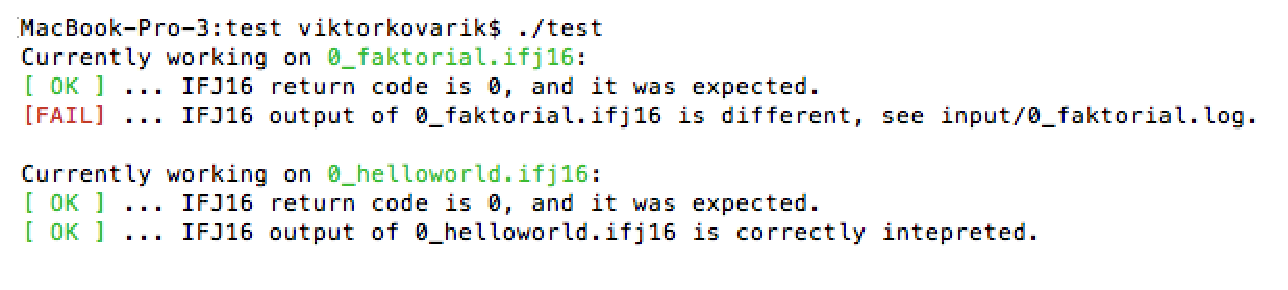
\includegraphics[width=0.7\linewidth]{testy-interpretu.eps}
%	\caption{}
%	\label{fig:testy-interpretu}
%\end{figure}

\begin{Verbatim}
ciUser@travis: ./test
Currently working on 0_ahojsvete.ifj16:
\textbf{\color{green}[ OK ]} ... IFJ16 return code is 0, and it was expected.
\textbf{\color{green}[ OK ]} ... IFJ16 output of 0_ahojsvete.ifj16 is correctly intepreted.

Currently working on 0_arithmetic_test_9_UNARY.ifj16:
\textbf{\color{red}[FAIL]} ... IFJ16 return code is 2, but 0 was expected, see logs/0_fooTest.log.
\textbf{\color{red}[FAIL]} ... IFJ16 output of 0_fooTest.ifj16 is different, see logs/0_fooTest.log.
\end{Verbatim}

\section{Přílohy}
\subsection{Diagramy konečného automatu lexikální analýzy}
\label{diag:LA-FSM}
\begin{figure}[H]
	\centering
	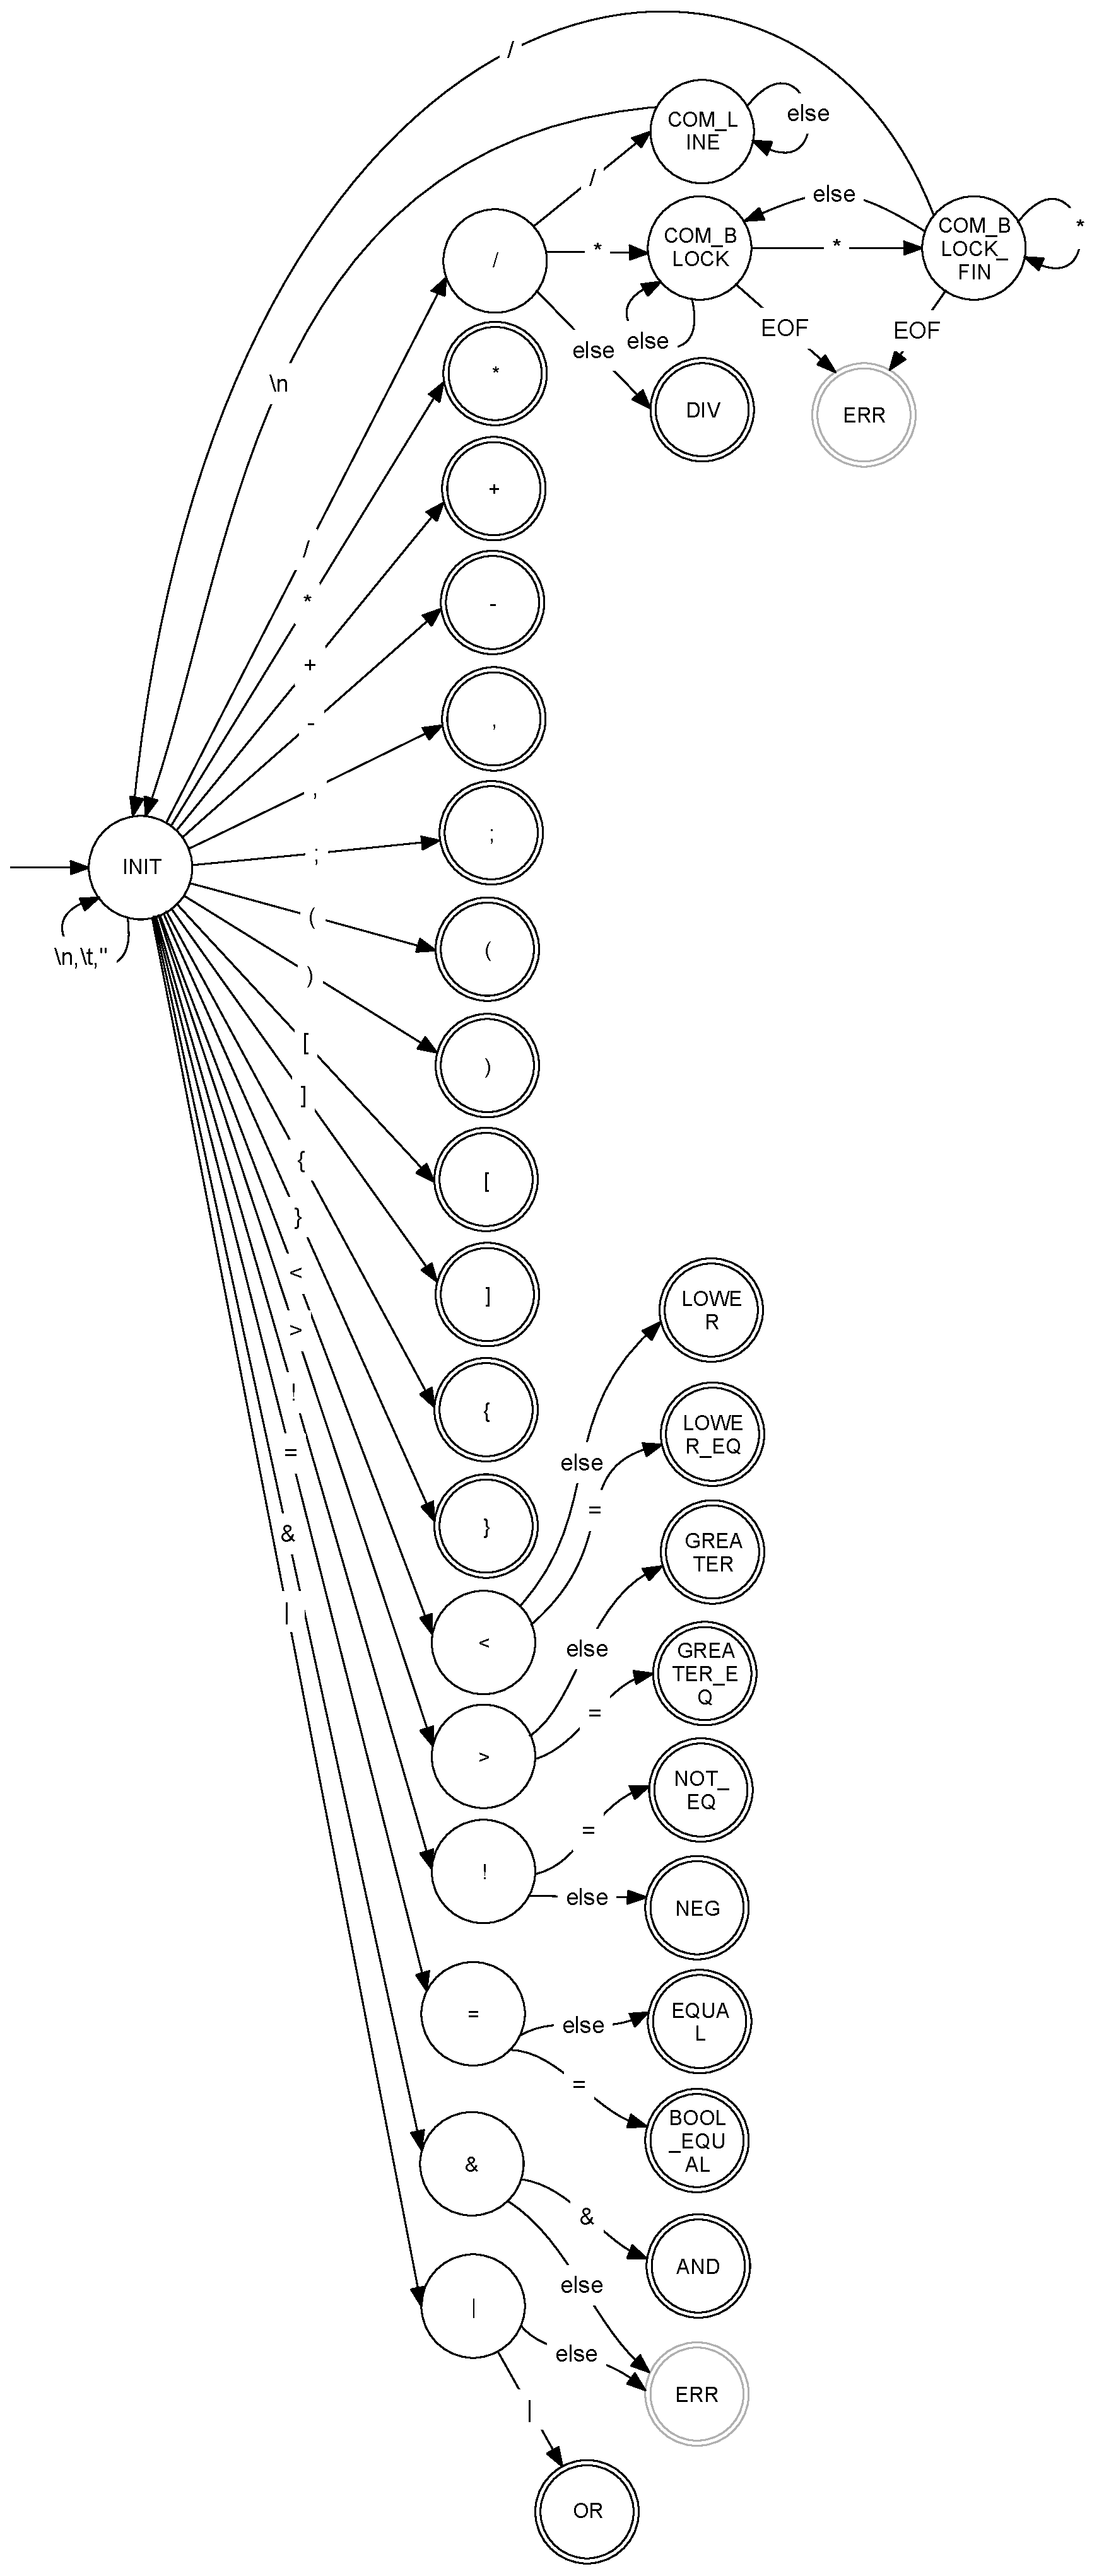
\includegraphics[scale=.31]{FSM_MAIN.eps}
	\caption{KA - hlavní schéma}
\end{figure}

\newpage
\begin{figure}[H]
	\centering
	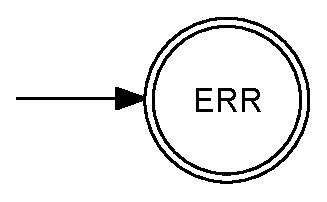
\includegraphics[scale=.31]{FSM_ERR.eps}
	\caption{KA - chyba}
\end{figure}

\begin{figure}[H]
	\centering
	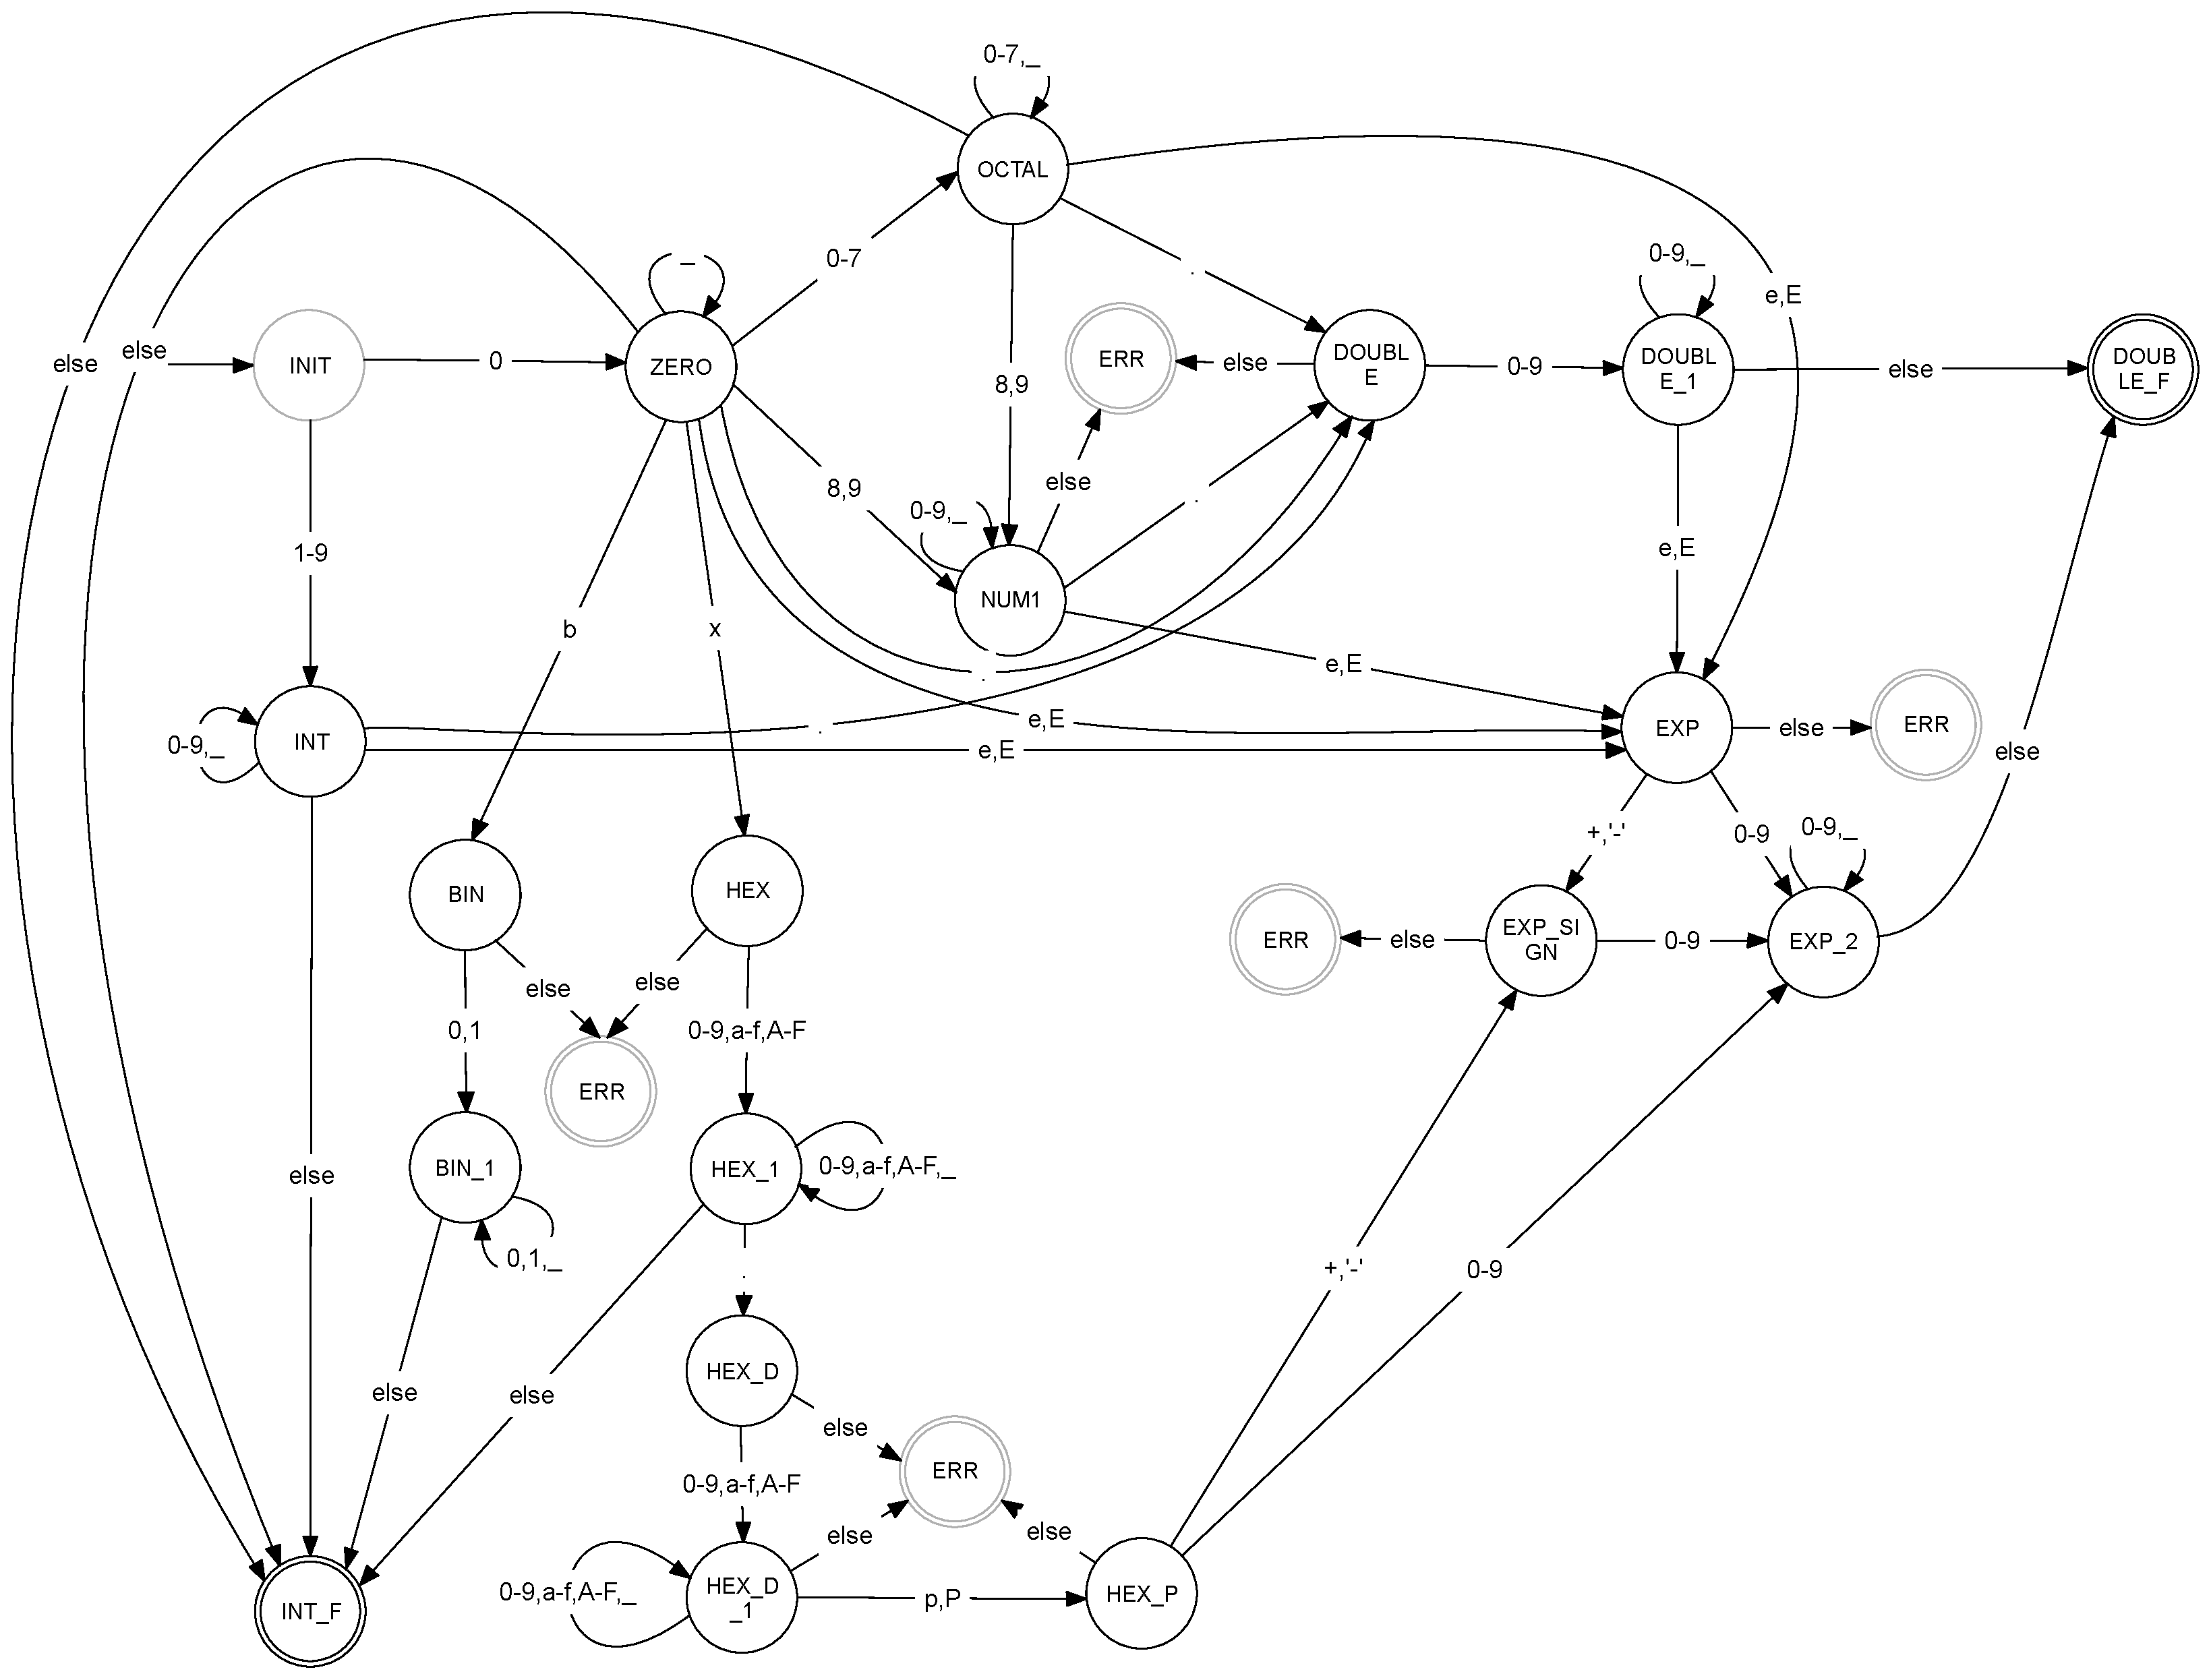
\includegraphics[scale=.308]{FSM_NUM.eps}
	\caption{KA - číslicový literál}
\end{figure}

\begin{figure}[H]
	\centering
	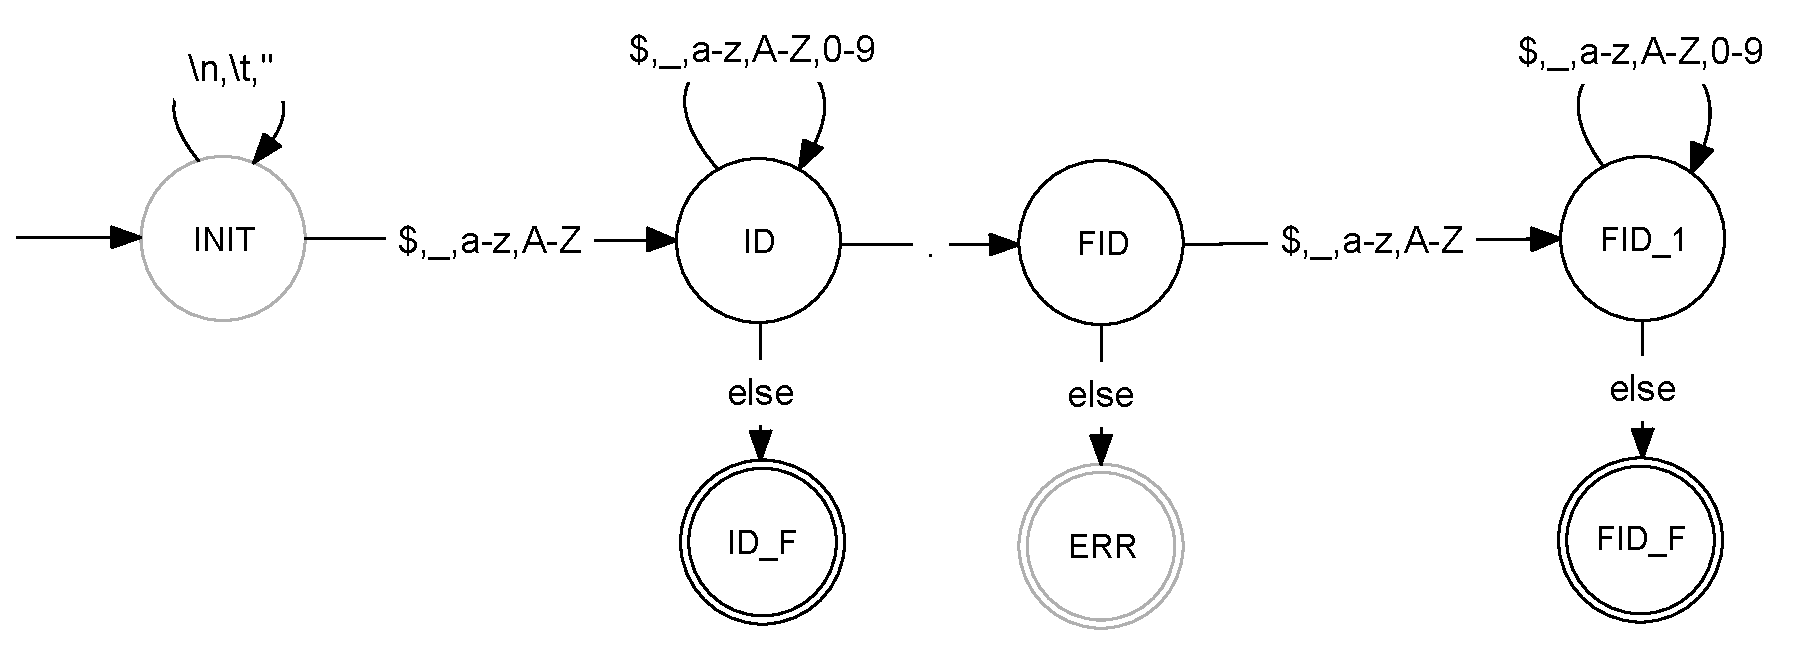
\includegraphics[scale=.31]{FSM_ID.eps}
	\caption{KA - identifikátor}
\end{figure}

\newpage
\begin{figure}[H]
	\centering
	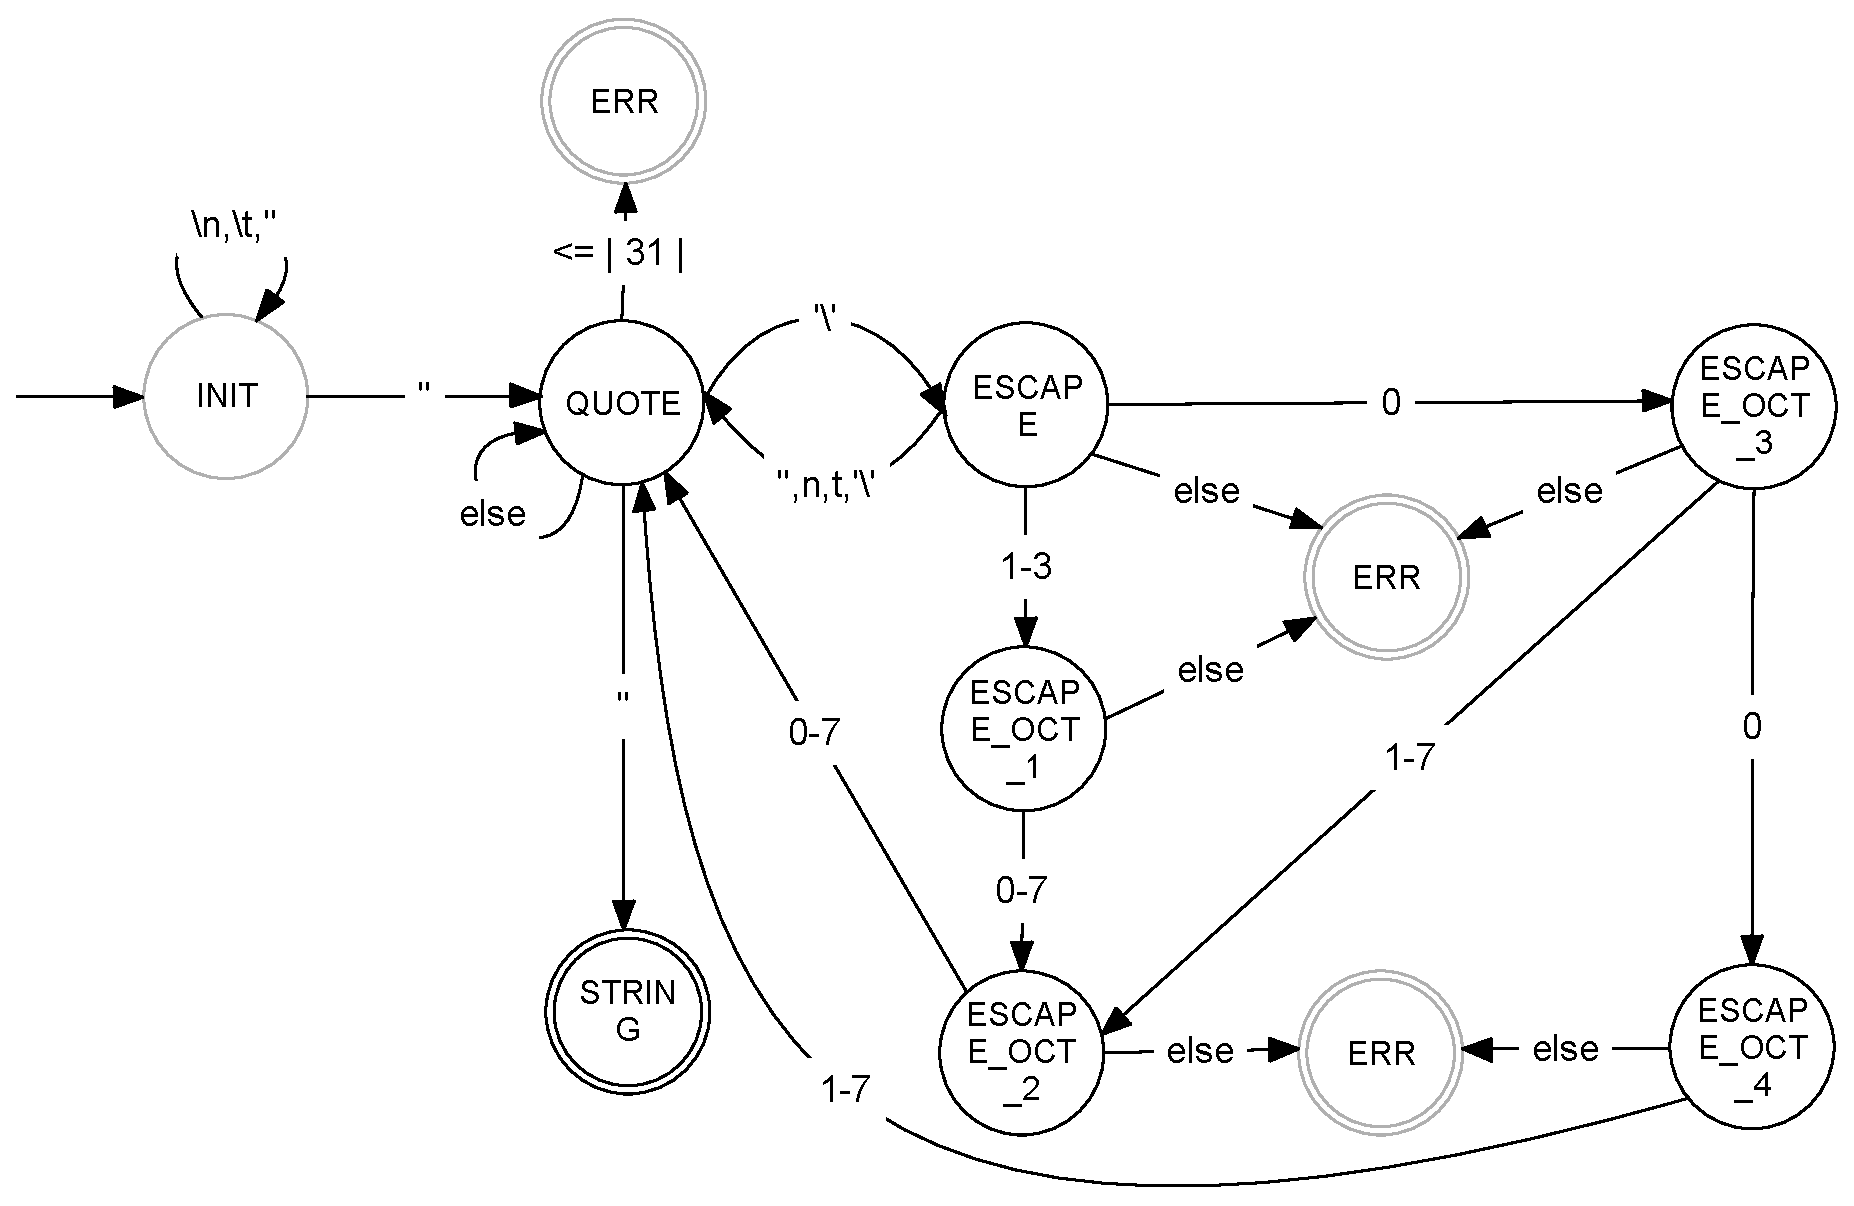
\includegraphics[scale=.31]{FSM_STRING.eps}
	\caption{KA - řetězec}
\end{figure}

\subsection{Precedenční tabulkaa}
\begin{figure}[H]
   \centering
   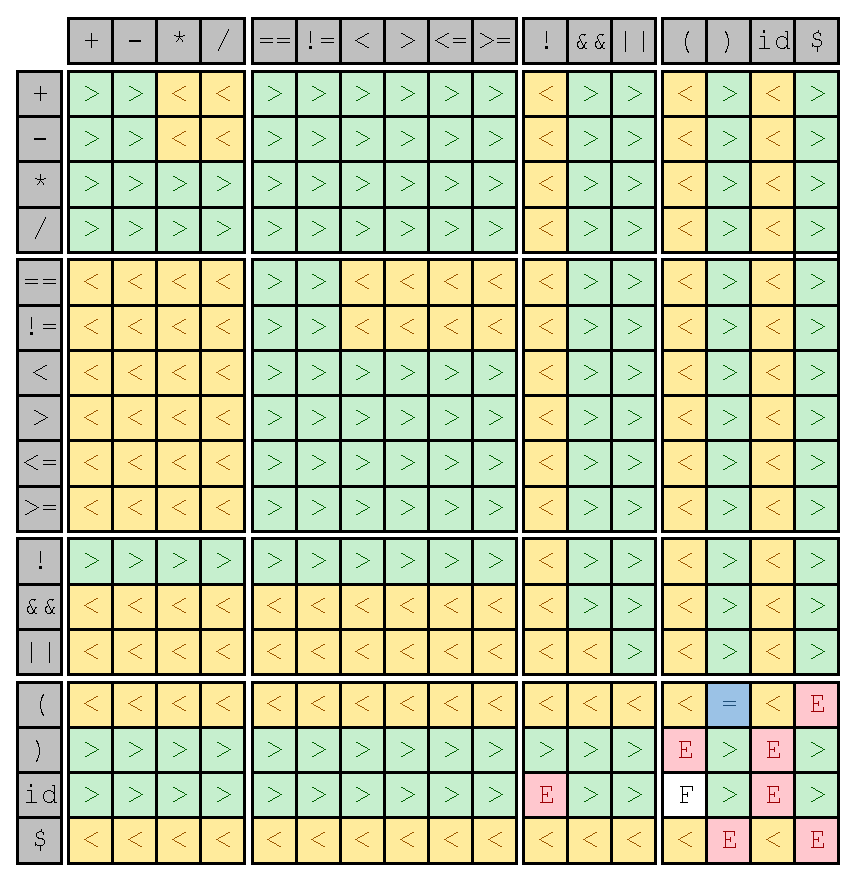
\includegraphics[]{precedence_tab.eps}
   \caption{Precedenční tabulka}
\end{figure}
\end{document}